% !TEX root = ReviewDraft.tex

The results  we reviewed above suggest that the black hole can be regarded as an ordinary system, obeying the laws of thermodynamics. More precisely, as an object 
  described by a finite, but large, number of degrees of freedom that obey the ordinary laws of physics, which in turn imply the laws of thermodynamics. 
   

In fact, this has been such an important idea in the development of the subject that we will call it the ``central dogma."   \begin{center}
{ \color{red} \underline{\bf%
 Central Dogma}}
\end{center}

 
{\center \begin{framed}   As seen from the outside, a black hole can be described in terms of a quantum system with  $  {\rm Area}/(4G_N ) $  degrees of freedom,   which evolves unitarily under time evolution. 
\end{framed}}
  

\begin{figure}[h]
\begin{center}
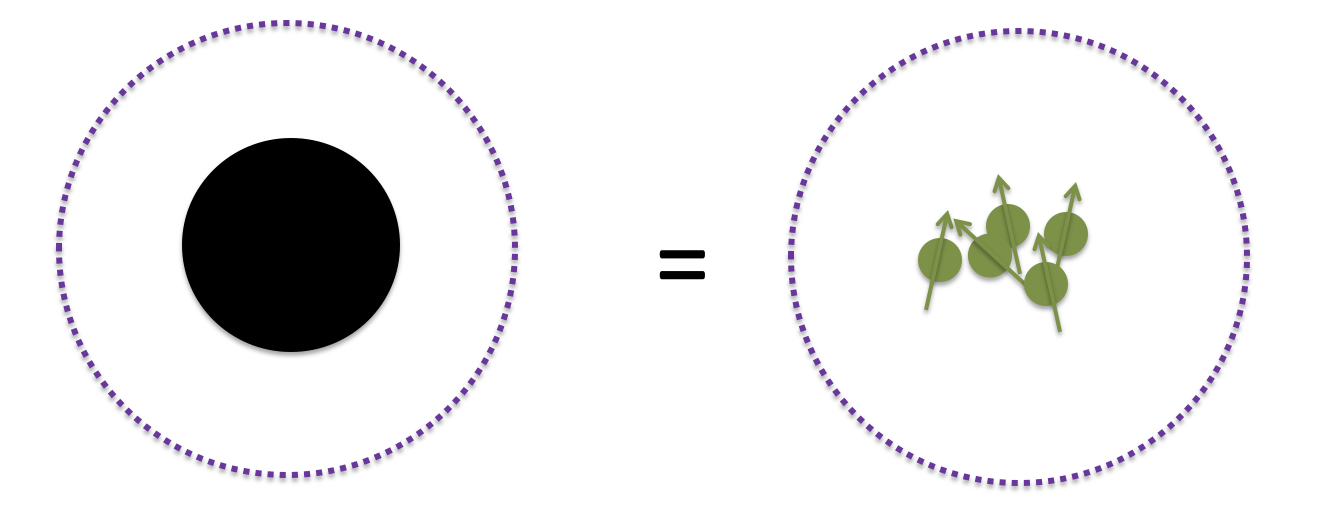
\includegraphics[scale=.3]{figures/BHQuantumBdy.png}
\caption*{Using this hypothesis, the black hole and the whole spacetime around it, up to some surface denoted by the dotted circle, can be replaced by a quantum system. This quantum system interacts with the outside via a unitary Hamiltonian. }
\label{BHQuantumBdy}
\end{center}
\end{figure}

 

Let us make some remarks about this. 
\begin{itemize}
	\item 
	Notice that it is a statement about the black hole as seen from the outside. There is no statement about the black hole interior, yet.  
\item
The statement about the number of degrees of freedom is primarily a statement about the logarithm of the dimension  of the Hilbert space. We make no distinction between qubits, fermions or other degrees of freedom. What is important is that the Hilbert space has {\it finite} dimension.   
\item
The degrees of freedom that appear in this statement are not manifest in the gravity description. Some researchers have tried to see them as coming from the thermal atmosphere, by putting a cutoff, or ``brick wall'' at some Planck distance from the horizon \cite{tHooft:1984kcu,Thorne:1986iy}. Unfortunately, such ideas remain vague since such cutoffs are not manifest from the gravity point of view, which treats the horizon as a smooth surface. 
\item
Unitary evolution implies that we have a Hamiltonian that generates the time evolution. Again, this Hamiltonian is not manifest in the gravity description. The gravity description has a Hamiltonian constraint, which determines the bulk evolution. But this constraint is a property of the full spacetime, we do not know how to pull out a purely exterior part.  
In principle, the Hamiltonian could  be very general. But the fact that it gives rise to the gravity evolution constrains some properties. For example, it should be strongly interacting and generate a very chaotic evolution. 
\item
We said that the black hole evolves unitarily.   This is when we surround the black hole by a reflecting wall and we consider the full system inside this wall. However, if the black hole lives in an asymptotically flat geometry, it is convenient to draw an imaginary surface surrounding the black hole and call everything inside the ``quantum system'' that appears in the central dogma. This quantum system is then coupled   with the external degrees of freedom living outside this surface.  We usually think of the region outside the imaginary surface as a quantum system in a fixed spacetime, where we ignore large fluctuations of the background, though  we can still consider weakly interacting gravitons.  The full coupled evolution should be unitary. In other words, in this context, the gravity answers are compared to those of a quantum system that is coupled to the degrees of freedom far from the black hole at this imaginary cutoff surface. Here we are imagining that this surface is at a few Schwarzschild radii from the black hole. 
\item
Often people ask: how is a black hole different from a hot piece of coal? This central dogma is saying that, as long as you remain outside, it is not fundamentally different, in the sense that both are governed by a unitary Hamiltonian and have a finite number of degrees of freedom. Unlike a piece of coal, the black hole has an interior shrouded by an event horizon, and making it fully compatible with the exterior view is a non-trivial problem that has not been completely solved. 
\item
The name ``central dogma'' was borrowed from biology where the central dogma talks about the information transfer from DNA and RNA to proteins. Here it is also a statement about information  $-$ quantum information. It involves a certain dose of belief, because it is not something we can derive directly from the gravity description.  We can view it as an unproven assumption about the properties of a full theory of quantum gravity. It is also something that is not accepted by some researchers. In fact,  Hawking famously objected to it. 
\item
Notice that this statement is in stark contrast with a naive reading of the spacetime geometry. The spacetime geometry can be viewed as having two ``asymptotic'' regions. One is the obvious region outside, and the other is the future region near the singularity. See figure \ref{BabyUniverse}. Of course, the semiclassical gravity theory does not tell us how to evolve past this singularity, or even whether such evolution makes sense. From this point of view the interior is something we cannot access from the outside, but there is no obvious reason why some quantum information could not be lost here. In other words, if a black hole is a ``hole in space'' where things can get in and get lost, then the central dogma would be FALSE. In fact, this is one reason why some people think it is indeed false.  
\item
Both the results on black hole thermodynamics, as well as the results on fine-grained entropies we will discuss later, are true properties of a theory of gravity coupled to quantum fields and do {\it not} require the validity of the central dogma.   In other words, we are not assuming the central dogma in this review $-$ we are providing evidence for it. 
\end{itemize}

\begin{figure}[h]
\begin{center}
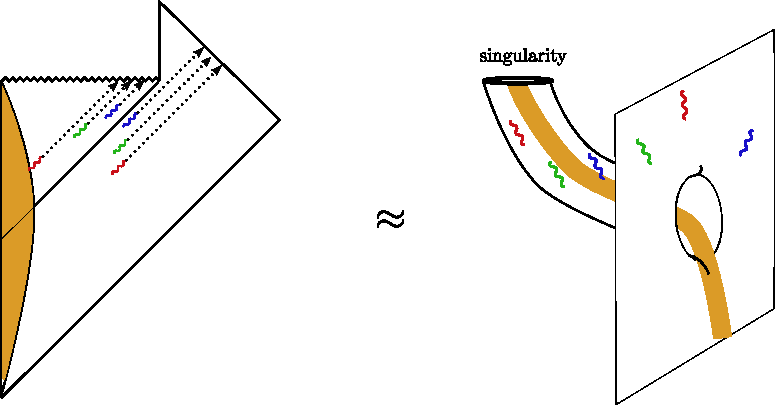
\includegraphics[scale=1]{figures/baby-universe.pdf} \\
(a) ~~~~~~~~~~~~~~~~~~~~~~~~~~~~~~~~~~~~~~~~~~~~~~~~~~~~~~~~~~~~~~~~~~~~~~~~~~~(b)
\caption{\small The skeptics' view: The diagram of an evaporating black hole is conceptually similar to one where we split off a baby universe, so that in the future we have two regions, the future region of the original universe, and the future of the interior, which is singular.}
\label{BabyUniverse}
\end{center}
\end{figure}


\subsection{Evidence from string theory for the central dogma} 

 
Though we said that the ``central dogma'' is an unproven assumption, there is a great deal of very non-trivial evidence from string theory. 
String theory is a modification of Einstein gravity that leads to a well defined perturbative expansion and also some non-perturbative results. For this reason it is believed to define a full theory of quantum gravity. 

One big piece of evidence was the computation of black hole entropy for special extremal black holes in supersymmetric string theories \cite{Strominger:1996sh}. In these cases one can reproduce the 
 Bekenstein-Hawking   formula from an explicit count of microstates.  These computations match not only the area formula, but all its corrections, see e.g. \cite{Dabholkar:2014ema}. Another piece of evidence comes from the AdS/CFT correspondence \cite{Maldacena:1997re,Witten:1998qj,Gubser:1998bc}, which is a conjectured relation between the physics of AdS and a dual theory living at its boundary.  In this case, the black hole and its whole exterior can be represented in terms of degrees of freedom living at the boundary. There is also evidence from matrix models that compute scattering amplitudes  in special vacua \cite{Banks:1996vh}.  We will not discuss this further  in this review, since we are aiming to explain features which rely purely on gravity as an effective field theory. 

\section{Fine-grained vs coarse-grained entropy} \label{finecoarse}

There are two notions of entropy that we ordinarily use in physics and it is useful to make sure that we do not confuse them in this discussion. 

The simplest to define is the von Neuman entropy. Given the density matrix, $\rho$,  describing the quantum state of the system, we have 
\be \label{vnfine}
S_{vN} = - Tr[ \rho \log \rho ] 
\ee
 It quantifies our ignorance about the precise quantum state of the system.    It vanishes for a pure state, indicating complete knowledge of the quantum state. An important property is that it is invariant under unitary time evolution $\rho \to U \rho U^{-1}$.  

The second notion of entropy  is the coarse-grained entropy. Here we have some density matrix $\rho$ describing the system, but we do not measure all observables, we only measure a subset of simple, or coarse-grained observables $A_i$. Then the coarse-grained entropy is given by the following procedure. We consider all possible density matrices $\tilde \rho$ which give the same result as our system for the observables that we are tracking, 
$Tr[ \tilde \rho A_i] =Tr[\rho A_i]$. Then we compute the von Neumann entropy $S(\tilde \rho)$. Finally we maximize this over all possible choices of $\tilde \rho$. 

Though this definition looks complicated, a simple example is the ordinary entropy used in thermodynamics. In that case the $A_i$ are often chosen to be a few observables, say the approximate energy and the volume. The thermodynamic entropy is obtained by maximizing the von Neumann entropy among all states with that approximate energy and volume. 

Coarse-grained entropy obeys the second law of thermodynamics. Namely, it  tends to increase under unitary time evolution. 

Let us make some comments.
\begin{itemize}
	\item The von Neumann entropy is sometimes called the ``fine-grained entropy'', contrasting it with the  coarse-grained entropy defined above. Another common name is  ``quantum entropy." 
	\item 
 Note that the generalized entropy defined in \nref{sgen} increases rapidly when the black hole first forms and the horizon grows from zero area to a larger area.   Therefore if it has to be one of these two entropies, it can only be the thermodynamic entropy. In other words, the entropy \eqref{sgen} defined as the area of the horizon plus the entropy outside is the coarse-grained entropy of the black hole. 
\item 
Note that if we have a quantum system composed of two parts $A$ and $B$, the full Hilbert space is $H= H_A \times H_B$. Then we can define the von Neumann entropy for the subsystem $A$.  This is computed  by first forming a density matrix $\rho_A$ obtained by taking a partial trace over the system $B$. The entropy of $\rho_A$ can be non-zero, even if the full system is in a pure state. This arises when the original pure state contains some entanglement between the subsystems $A$ and $B$. 
In this case $S(A)=S(B)$ and $S(A\cup B) =0$. 
\item
The fine-grained entropy cannot be bigger than the coarse-grained entropy, $S_{vN} \leq S_{coarse}$. 
 This is a simple consequence of the definitions, since we can always consider $\rho$ as a candidate $\tilde \rho$. Another way to say this is that because $S_{coarse}$ provides a measure of the total number of   degrees of freedom available to  the system, it sets an upper bound on how much the system can be entangled with something else.




  
 \end{itemize}


It is useful to define the fine-grained entropy of the quantum fields in a region of space. Let $\Sigma$ be a spatial region, defined on some fixed time slice. This region has an associated density matrix $\rho_{\Sigma}$, and the fine-grained entropy of the region is denoted
\be
 S_{vN}(\Sigma) \equiv S_{vN}(\rho_\Sigma) \ .
\ee
If $\Sigma$ is not a full Cauchy slice, then we will have some divergences at its boundaries. These divergences are not important for our story, they have simple properties and we can deal with them appropriately.  Also, when $\Sigma$ is a portion of the full slice,   $S_{vN}(\Sigma)$ is generally time-dependent. It can increase or decrease with time as we move the slice  forwards   in time. The slice $\Sigma$ defines an associated causal diamond, which is the region that we can determine if we know initial data in $\Sigma$, but not outside $\Sigma$. The entropy is the same for any other slice $\tilde \Sigma$ which has the same causal diamond as $\Sigma$, see figure \ref{Diamond}.  



\begin{figure}[h]
\begin{center}
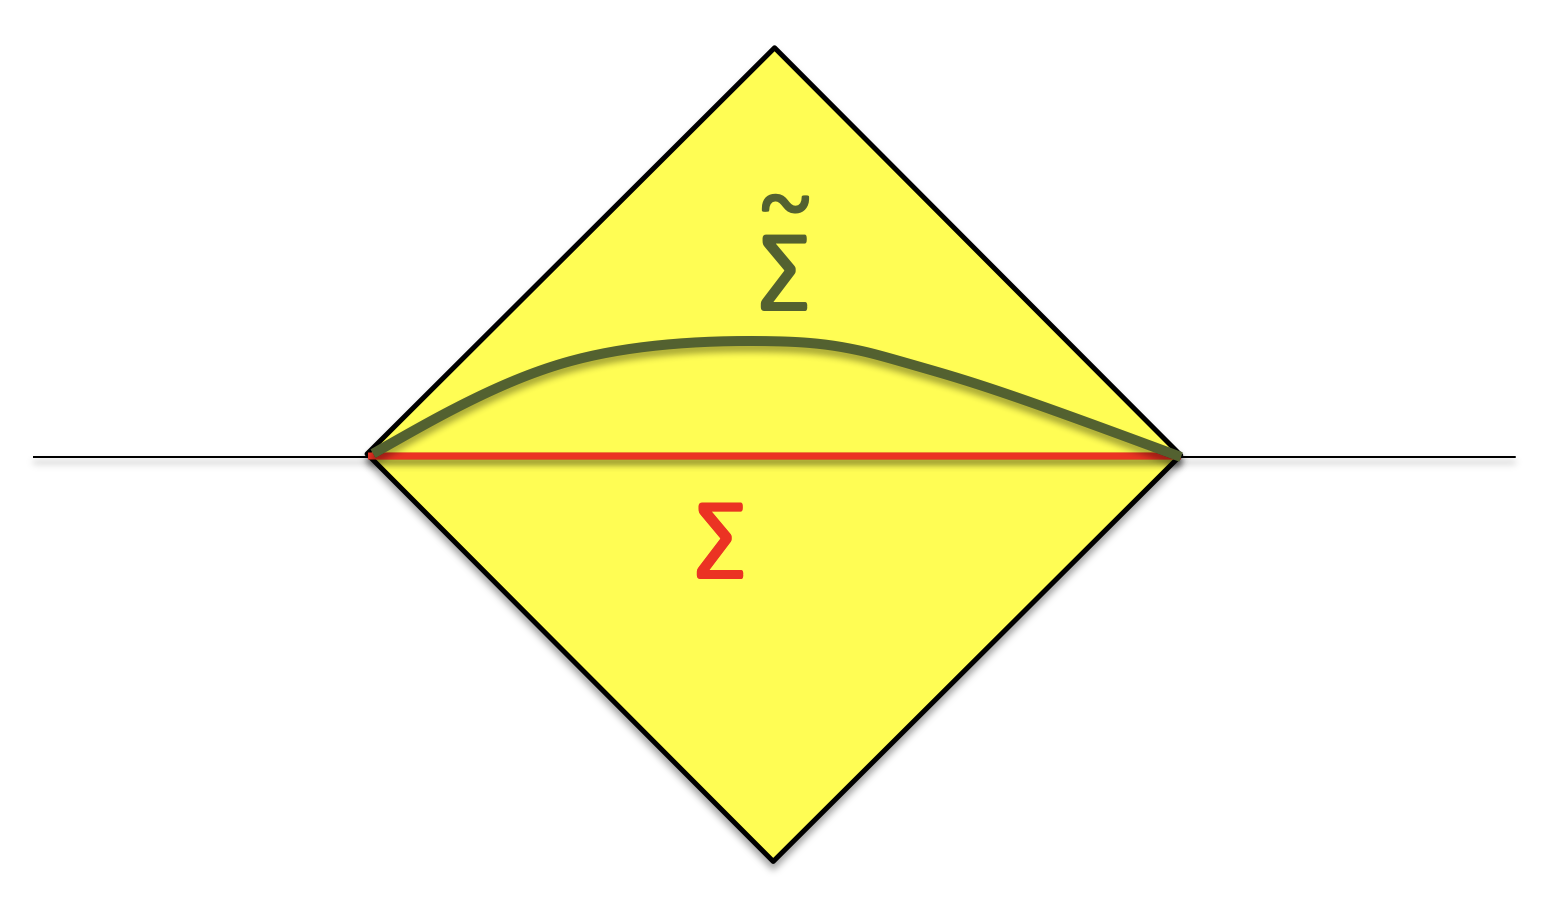
\includegraphics[scale=.3]{figures/Diamond.png}
\caption{ Given a region $\Sigma$ of a spatial slice, shown in red, we can define its causal diamond to be all points where the evolution is uniquely  determined by initial conditions on $\Sigma$. The alternative slice $\tilde \Sigma$ defines the same causal diamond. The von Neumann entropies are also the same.  }
\label{Diamond}
\end{center}
\end{figure}




\subsection{Semiclassical entropy}\label{semiclassical}

We now consider a gravity theory which we are treating in the semiclassical approximation. Namely, we have a classical geometry and quantum fields defined on that classical geometry. 
Associated to a spatial subregion we can define its 
 ``semiclassical entropy,"    denoted by
\be
\Ssemi(\Sigma) \ .
\ee
$\Ssemi$ is the von Neumann entropy of quantum fields (including gravitons) as they appear on the semiclassical geometry. In other words, this is the fine-grained entropy of the density matrix calculated by the standard methods of quantum field theory in curved spacetime. In the literature, this is often simply called the von Neumann entropy (it is also called $S_{\rm matter}$ or $S_{\rm outside}$ in the black hole context).

 


\section{The Hawking information paradox }

The   Hawking information paradox is an argument against the ``central dogma'' enunciated above \cite{Hawking:1976ra}. It is only a  paradox if we think that the central dogma is true.
 Otherwise, perhaps it can be viewed as a feature of quantum gravity.   

The basic point rests on an understanding of the origin of Hawking radiation. We can first start with the following question. Imagine that we make a black hole from the collapse of a pure state, such as a large amplitude gravity wave \cite{Christodoulou:2008nj}. This black hole emits thermal radiation. Why do we have these thermal aspects if we started with a pure state? The thermal aspects of Hawking radiation arise because we are essentially splitting the original vacuum state into two parts, the part that ends up in the black hole interior and the part that ends up in the exterior. The vacuum in quantum field theory is an entangled state. As a whole state it is pure, but the degrees of freedom are entangled at short distances. This implies that if we only consider half of the space, for example half of flat space, we will get a mixed state on that half. This is a very basic consequence of unitarity and relativistic invariance \cite{Bisognano:1976za}. 
 Often this is explained qualitatively as follows. The vacuum contains pairs of particles that are constantly being created and annihilated. In the presence of a horizon, one of the members of the pair can go to infinity and the other member is trapped in the black hole interior.  We will call them the ``outgoing Hawking quantum" and the ``interior Hawking quantum."  These two particles are entangled with each other, forming a pure state. However if we consider only one member, say the outgoing Hawking quantum, we fill find it in a mixed state, looking like a thermal state at the Hawking temperature \nref{thawking}. See figure \ref{fig:evap-stages}b and figure \ref{fig:evap-penrose}.
 
 
 This process on its own does not obviously violate the central dogma. In fact, if we had a very complex quantum system which starts in a pure state, it will appear to thermalize and will emit radiation that is very close to thermal. In particular, in the early stages, if we computed the von Neumann entropy of the emitted radiation it would  be almost exactly thermal because the radiation is entangled with the quantum system. So it is reasonable to expect that during the initial stages of the evaporation, the entropy of radiation rises. However, as the black hole evaporates more and more, its area will shrink and we run into trouble when the entropy of radiation is bigger than the thermodynamic entropy of the black hole. The reason is that now it is not possible for the entropy of radiation to be entangled with the quantum system describing the black hole because the number of degrees of freedom of the black hole is given by its thermodynamic entropy, the area of the horizon.
 In other words, if the black hole degrees of freedom together with the radiation  are producing a pure state, then the fine-grained entropy of the black hole should be equal to that of the radiation $S_{\rm black ~hole} = S_{\rm rad}$. But this fine-grained entropy of the black hole should be less than the Bekenstein-Hawking or thermodynamic entropy of the black hole, 
 $S_{\rm black~hole} \leq S_{\rm Bekenstein-Hawking}=S_{\rm coarse-grained}$. 
 % together with the d
 % A mixed state with entropy $S_{rad} $ cannot form a pure state (or be purified) by a system with coarse-grained entropy $S_{BH}$ if $S_{rad} > S_{BH}$. The reason is that if the black hole is purifying the radiation its fine-grained entropy should be at least that of the radiation. 
% At this point we run into a problem. 
 %\edgar{I think we want to rephrase the argument above to make clear the paradox is: $S_{rad}^{fine} > S_{BH} \defeq S_{BH}^{coarse} \geq S_{BH}^{fine}$. If we want we can furthermore use Page's result to say this is a sharp pinpointing of the problem, since $S_{coarse}^{BH} \approx S_{fine}^{BH}$ once $S_{rad}^{fine} > S_{BH}$.}
 
 If the central hypothesis were true, we would expect that the entropy of radiation would need to start decreasing at this point. In particular, it can never be bigger than the Bekenstein Hawking entropy of the old black hole. Notice that we are talking about the von Neumann or fine-grained entropy of the radiation. 
 Then, 
 as suggested by D. Page \cite{Page:1993wv,Page:2013dx}, the entropy of the radiation would need to follow the curve indicated in figure \ref{HawkingPageCurves}, as opposed to the Hawking curve.
 The time at which $S_{\rm Bekestein-Hawking} = S_{\rm rad}$ is called the Page time.
 
 \begin{figure}[h]
\begin{center}
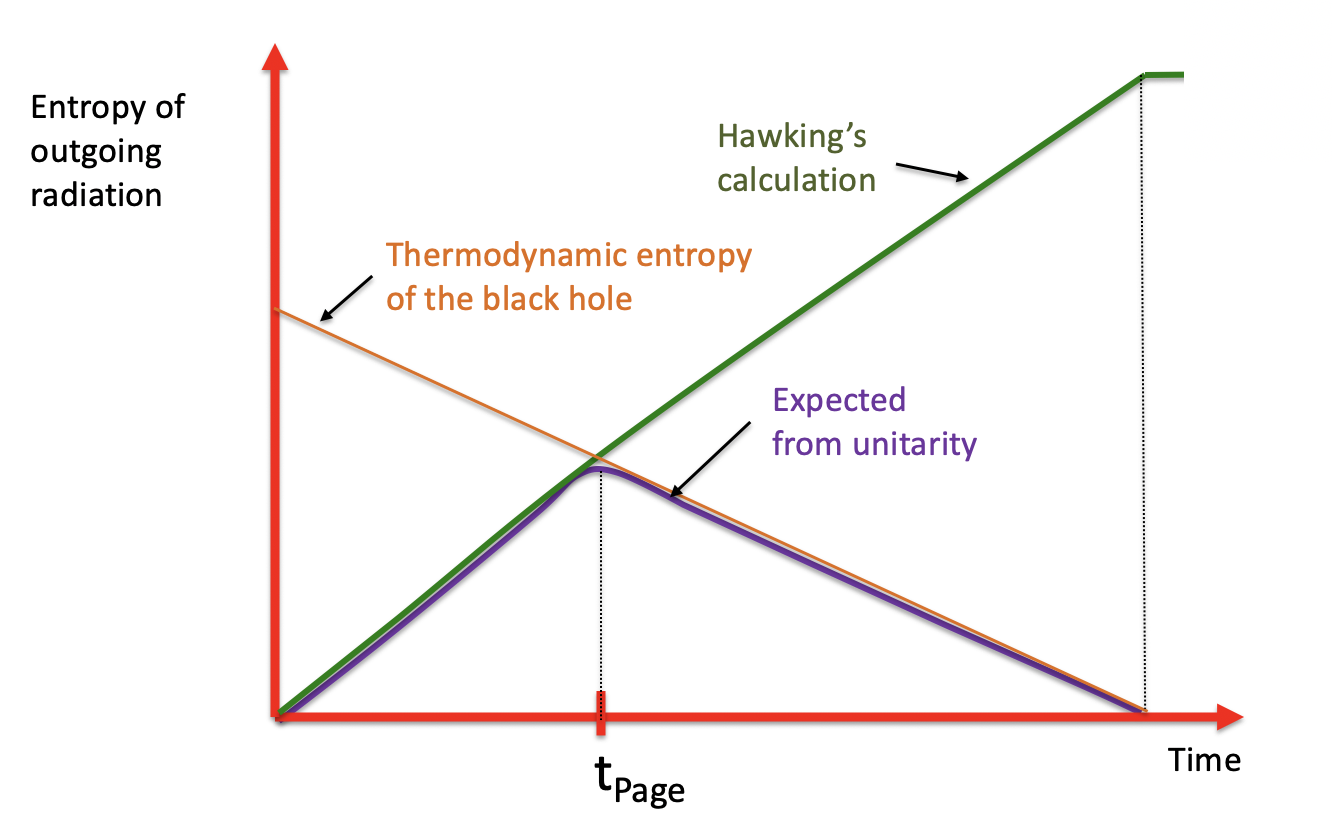
\includegraphics[scale=.5]{figures/BHPage.png}
\caption{  Schematic behavior of the entropy of the the outgoing radiation.  The precise shape of the lines depends on the black hole and the details of the matter fields being radiated.  In green we see Hawking's result, the entropy monotonically increases until $t_{\rm End}$, when the black hole completely evaporates. In orange we see the thermodynamic entropy of the black hole. If the process is unitary, we expect the entropy of radiation to be smaller than the thermodynamic entropy. If it saturates this maximum, then it should follow the so called ``Page'' curve, denoted in purple. This changes relative to the Hawking answer at the Page time, $t_{\rm Page}$, when the entropy of Hawking radiation is equal to the thermodynamic entropy of the black hole.  }
\label{HawkingPageCurves}
\end{center}
\end{figure}
 
 Now let us finish this discussion with a few comments. 
 
 \begin{itemize}
 \item
 Note that, as the black hole evaporates, its mass decreases. This is sometimes called the ``backreaction'' of Hawking radiation. This effect is included in the discussion. And it does not ``solve'' the problem.
 \item
 When the black hole reaches the final stages of evaporation, its size becomes comparable to the Planck length and we can no longer trust the semiclassical gravity description.  This is not relevant since the conflict with the central dogma appeared at the Page time, when the black hole was still very big. 
 \item The argument is very robust since it relies only on basic properties of the fine-grained entropy. In particular, it is impossible to fix the problem by adding small corrections to the Hawking process by slightly modifying the Hamiltonian or state of the quantum fields near the horizon \cite{Mathur:2009hf,Almheiri:2012rt,Almheiri:2013hfa}.  In other words, the paradox holds to all orders in perturbation theory, and so if there is a resolution it should be non-perturbative in the gravitational coupling $\GN$.
 \item
 We could formulate the paradox by constantly feeding the black hole with a pure quantum state	so that we exactly compensate the energy lost by Hawking radiation. Then the mass of the black hole is constant. Then the paradox would arise when this process goes on for a sufficiently long time that the entropy of radiation becomes larger than the entropy of the black hole. 
 \item
 One could say that the gravity computation only gives us an approximate description and we should not expect that a sensitive quantity like the von Neumann entropy should be exactly given by the  semiclassical theory. In fact, this is what was said until recently. We will see however, that there \emph{is} a way to compute the von Neuman entropy using just this semiclassical description. 
 \end{itemize}


 We have described here one aspect of the Hawking information paradox, which is the aspect that we will see how to resolve. We will comment about other aspects in the discussion.  
 
